
%
% state - vis
%

\section{Visual mapping}

N\"{o}llenburg~\cite{noellenburg11geovis} names three ``Driving forces in geovisualization'': The advent of high speed parallel processing and technology advances in computer graphics, today allows us to grasp enormous amounts of information. Besides the advances in graphics and display technologies, the second main driving force in geographic visualization is the increasing amount of geospatial data being collected and available. Finally, the third force is the \textit{rise of the Internet}, which significantly pushes web mapping and contributes to geovisualization technologies.

As a logical consequence of broader audiences having access to geospatial visualizations using the Internet, it appears that there is a shift from technology-driven visualization towards more human-centered approaches. Interactive and highly dynamic interfaces have helped the map evolve from its traditional role as a presentational device towards exploring geospatial data~\cite{noellenburg11geovis, vislecture}.

In chapter \ref{chapter:foundations-vis}, foundations of visualization, visual variables and data exploration techniques as well as the concept of clutter reduction have been introduces. In the following, existing visualization techniques for representing clustered data on maps will be discussed. In a first step, visualization concepts on the map level will be discussed. Later, approaches for visualizing individual clusters will are added. 

\subsection{Map visualization types for clustering}
\label{chapter:map-vis}

There exists a variety of map types, serving different purposes like standard geographic maps, cartograms, geologic maps, linguistic maps or weather maps. Some of these use distortion, for example the cartogram can be used to map the area of each country to the size of population. In this section, we try to identify those map types which are appropriate for visualizing clustered data\cite{noellenburg11geovis, wiki:map-types}:

\begin{itemize}

\item \textbf{Geographic map with markers}. The default way of representing data is a standard 2-dimensional map with markers on top of it. Each marker represents a data point or in the case of clustering, a cluster.

\parbox [h]{0.4\textwidth}{
    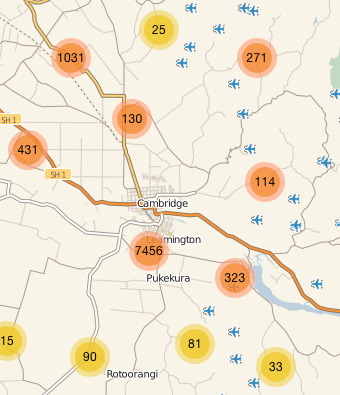
\includegraphics [width=\linewidth]{figures/map_types_normal_leaflet.png}
    \captionof {figure}{Leaflet map}
    \label{fig:map-type-standard-leaflet}
}
\hfill
\hspace{0.5cm}
\parbox [h]{0.4\textwidth }{
    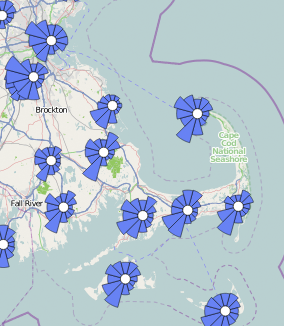
\includegraphics [width=\linewidth]{figures/map_types_standard_wind.png}
    \captionof {figure}{Wind history map}
    \label{fig:map-type-standard-wind}
}

\begin{itemize}

\item Figure \ref{fig:map-type-standard-leaflet} depicts an example\footnote{Leaflet.clustermarker example map from \url{http://leaflet.github.io/Leaflet.markercluster/example/marker-clustering-realworld.10000.html}} of the Leaflet.markercluster library. Clustered results are displayed using markers of the same size. The amount of items within a cluster is indicated by using a ``hot-to-cold'' color ramp~\cite{web:color-ramp}. 

\item Figure \ref{fig:map-type-standard-wind} shows a similar example, in this case a Wind history map\footnote{Wind history map \url{http://windhistory.com/map.html}} with markers for every wind measurement point. In this case, an advanced visualization technique is used for visualizing the amount of wind per cardinal direction as polar area diagrams.

\end {itemize}

The comparison between the two standard maps shows the potential of using advanced visualization techniques for displaying cluster items. Further ways for cluster visualization will be discussed in chapter \ref{chapter:cluster-vis}.

\item \textbf{Geographic Heatmap}

Heatmaps use colored, two-dimensional areas to express the value of each data entity on the map. Choropleth maps are the most common heatmaps, which are often used for analysis of geographic and statistical data. 

\parbox [h]{0.4\textwidth}{
    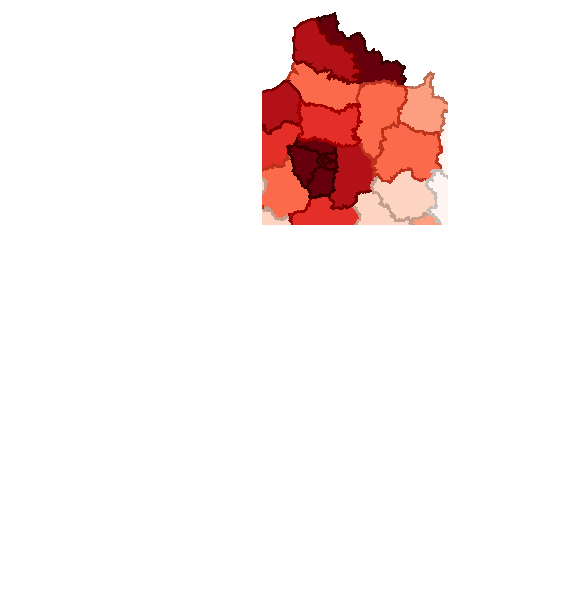
\includegraphics [width=\linewidth]{figures/map_types_choropleth.pdf}
    \captionof {figure}{Choropleth map}
    \label{fig:map-type-choropleth}
}
\hfill
\hspace{0.5cm}
\parbox [h]{0.4\textwidth}{
    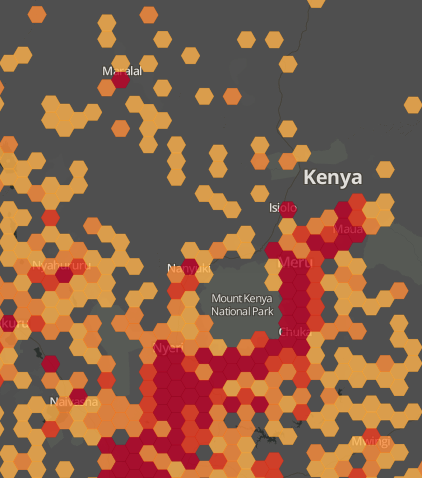
\includegraphics [width=\linewidth]{figures/map_types_heatmap.png}
    \captionof {figure}{Heatmap}
    \label{fig:map-type-binning}
}


\begin{itemize}

\item Figure \ref{fig:map-type-choropleth} visualizes an example choropleth map\footnote{Choropleth map example from Kartograph \url{http://kartograph.org/showcase/choropleth/}} that shows population data for each of the departments of metropolean France. Color coding is used to indicate densely populated regions with heavier red tones.

\item Figure \ref{fig:map-type-binning} presents another example\footnote{Heatmap that uses binning \url{http://mapbox.com/blog/binning-alternative-point-maps/}} that uses \textit{binning} for creating a hexagonal tessellation of the surface in order to visualize clustered results. 

\end {itemize}

A problem with heat maps is that they require a non-overlapping tessellation of the surface to provide the areas for visualization. As the binning example indicates, such a tessellation can also be done programmatically. Heatmap therefore can also be used for visualizating arbitrary clustered data without a need to calculate the exact boundaries of clusters. Another variation of heatmaps is the prism map, which adds extrusion of areas as a third-dimension~\cite{ladenhauf12dia, Delort10vis}. A publication on the evaluation of color schemes in choropleth maps can be found in~\cite{MacEachrenMort}. 


\item \textbf{Dot Grid maps}

Dot Grid maps are based on the suggestion by Jaques Bertin~\cite{bertin67graphics, bertin83graphics} to use graduated sizes in a regular pattern as an alternative to chloropeth maps. The advantage is, that the map creator doesn't have to choose between quantity or density of a distribution value, because the dot grid map shows both a the same time. The user can understand the data distribution on a finer level of granularity, as opposed to where the chloropeth map usually creates larger areas of aggregated information~\cite{web:dot-grid}.

Figure \ref{fig:map-type-dotgrid} is an alternative version\footnote{Dot Grid map example from Kartograph \url{http://kartograph.org/showcase/dotgrid/}} of the France map from figure \ref{fig:map-type-choropleth}, visualized as a dot grid map.


\item \textbf{Voronoi map}

The Voronoi tessellation is a space partitioning technique. From a set of points, it produces a Voronoi polygon for each point, such that the area covered is closest to that point in comparison to all other points. Jean-Yves Delort describes a technique that uses Voronoi polygons for ``Vizualizing Large Spatial Datasets in Interactive Maps''~\cite{Delort10vis}. It uses a hierarchical clustering technique to choose a subset of points per zoom level for proper visualization. Still, the effectiveness of this approach is questionable, as the scalability analysis of the studies shows that the technique can efficiently be used for datasets of up to 1000 items.

Figure \ref{fig:map-type-voronoi} show an exemplary voronoi map\footnote{Voronoi map example \url{http://mbostock.github.io/d3/talk/20111116/airports-all.html}} that displays all U.S. airports as of 2008. Besides the shown visualization, for Voronoi maps apply the same visualization possibilities as for cloropeth maps.

\parbox [h]{0.4\textwidth }{
    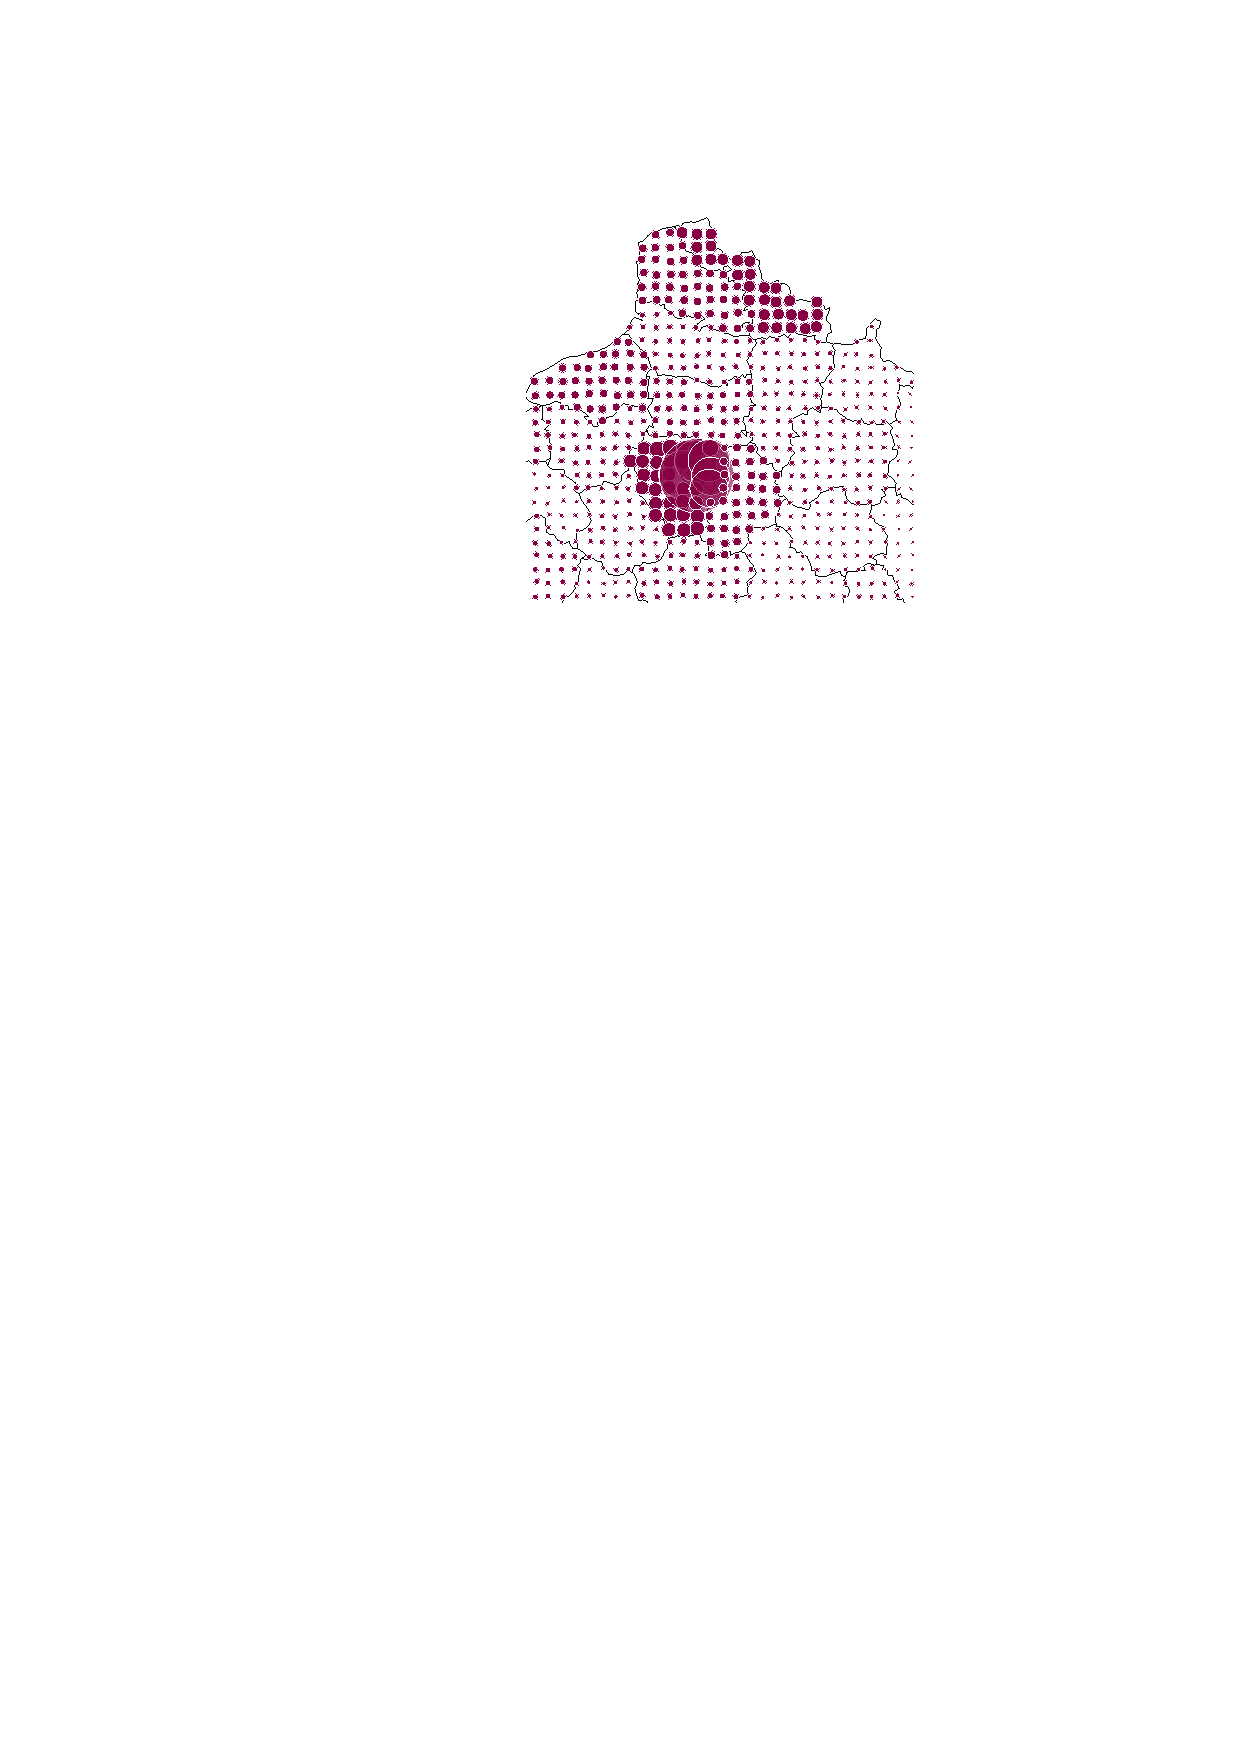
\includegraphics [width=\linewidth]{figures/map_types_dot_grid.pdf}
    \captionof {figure}{Dot Grid map}
    \label{fig:map-type-dotgrid}
}
\hfill
\hspace{0.5cm}
\parbox [h]{0.4\textwidth }{
    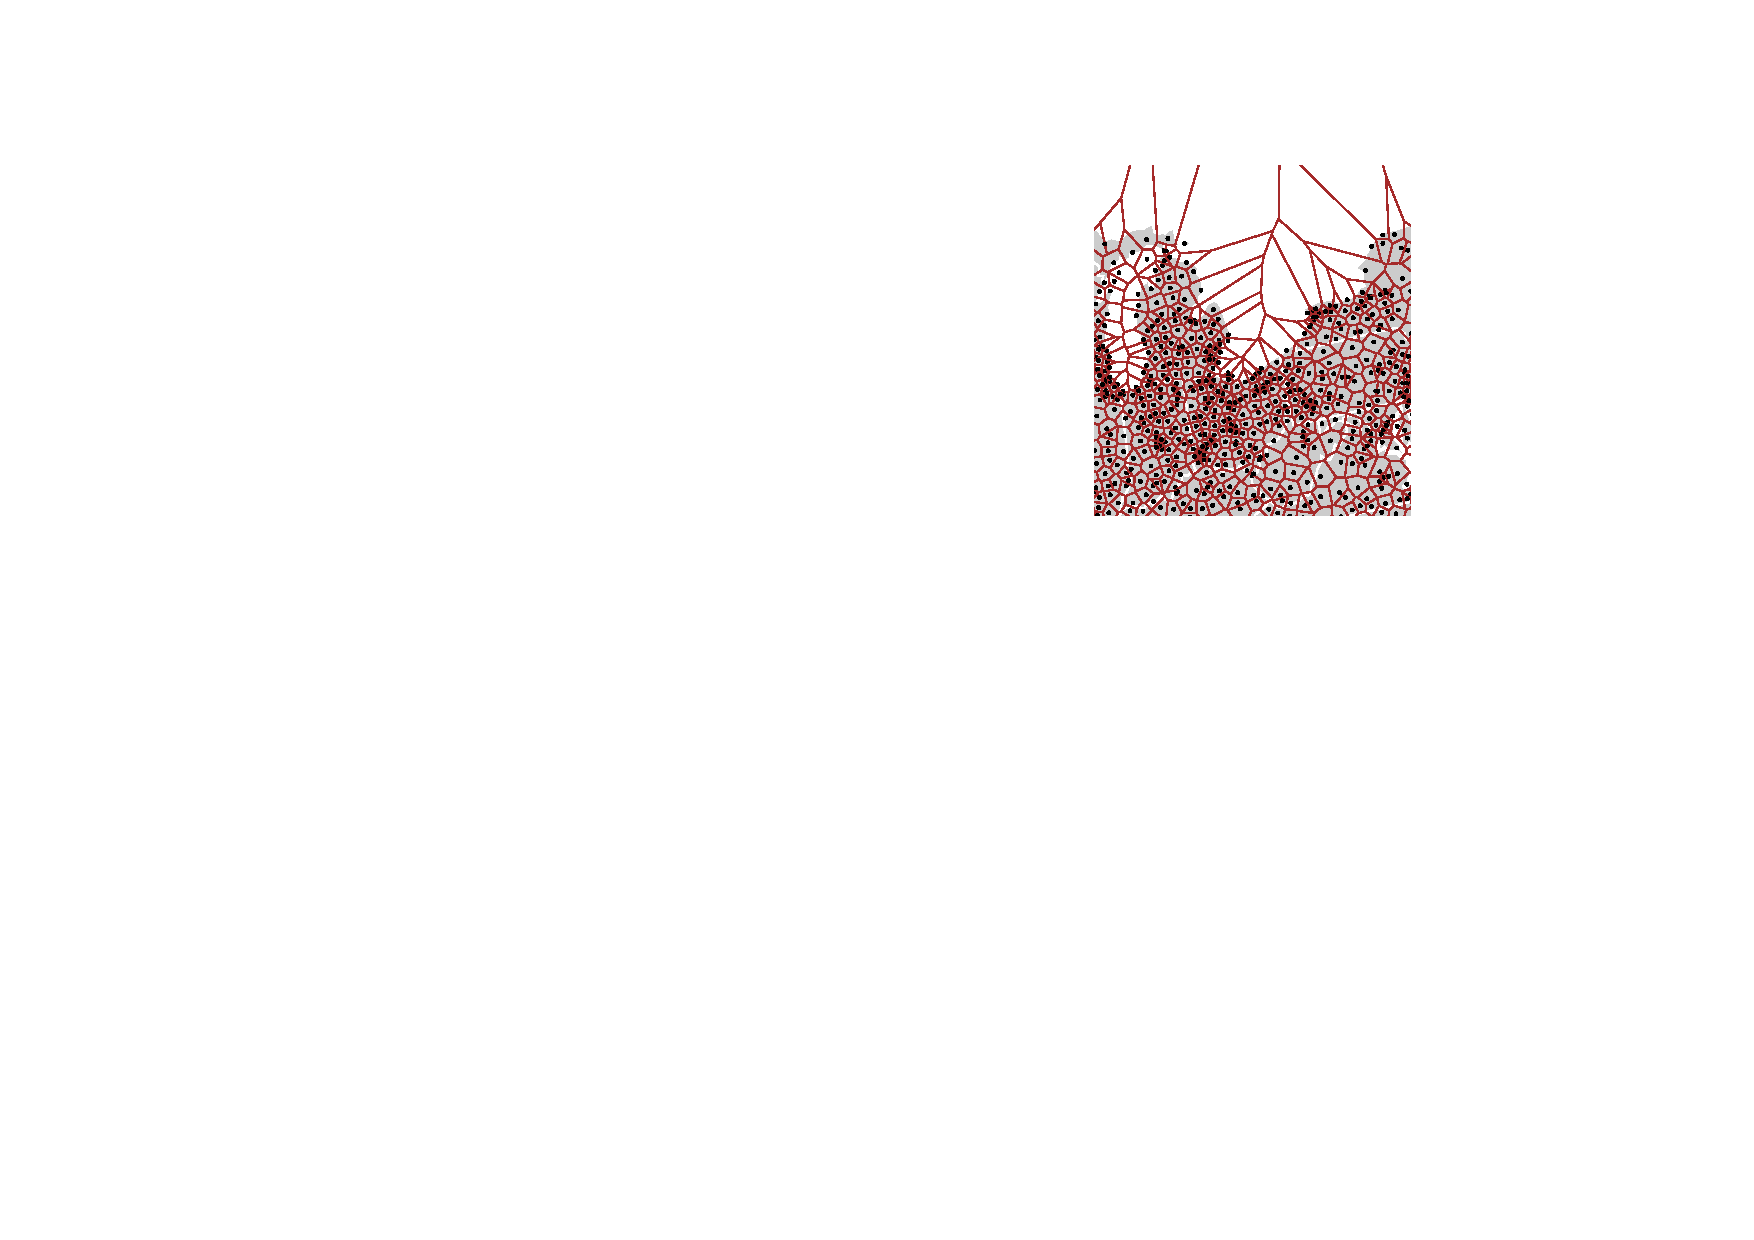
\includegraphics [width=\linewidth]{figures/map_types_voronoi.pdf}
    \captionof {figure}{Voronoi map}
    \label{fig:map-type-voronoi}
}

\end{itemize}

\subsection{Cluster visualization techniques}
\label{chapter:cluster-vis}



\begin{figure}[h]
  \begin{center}
    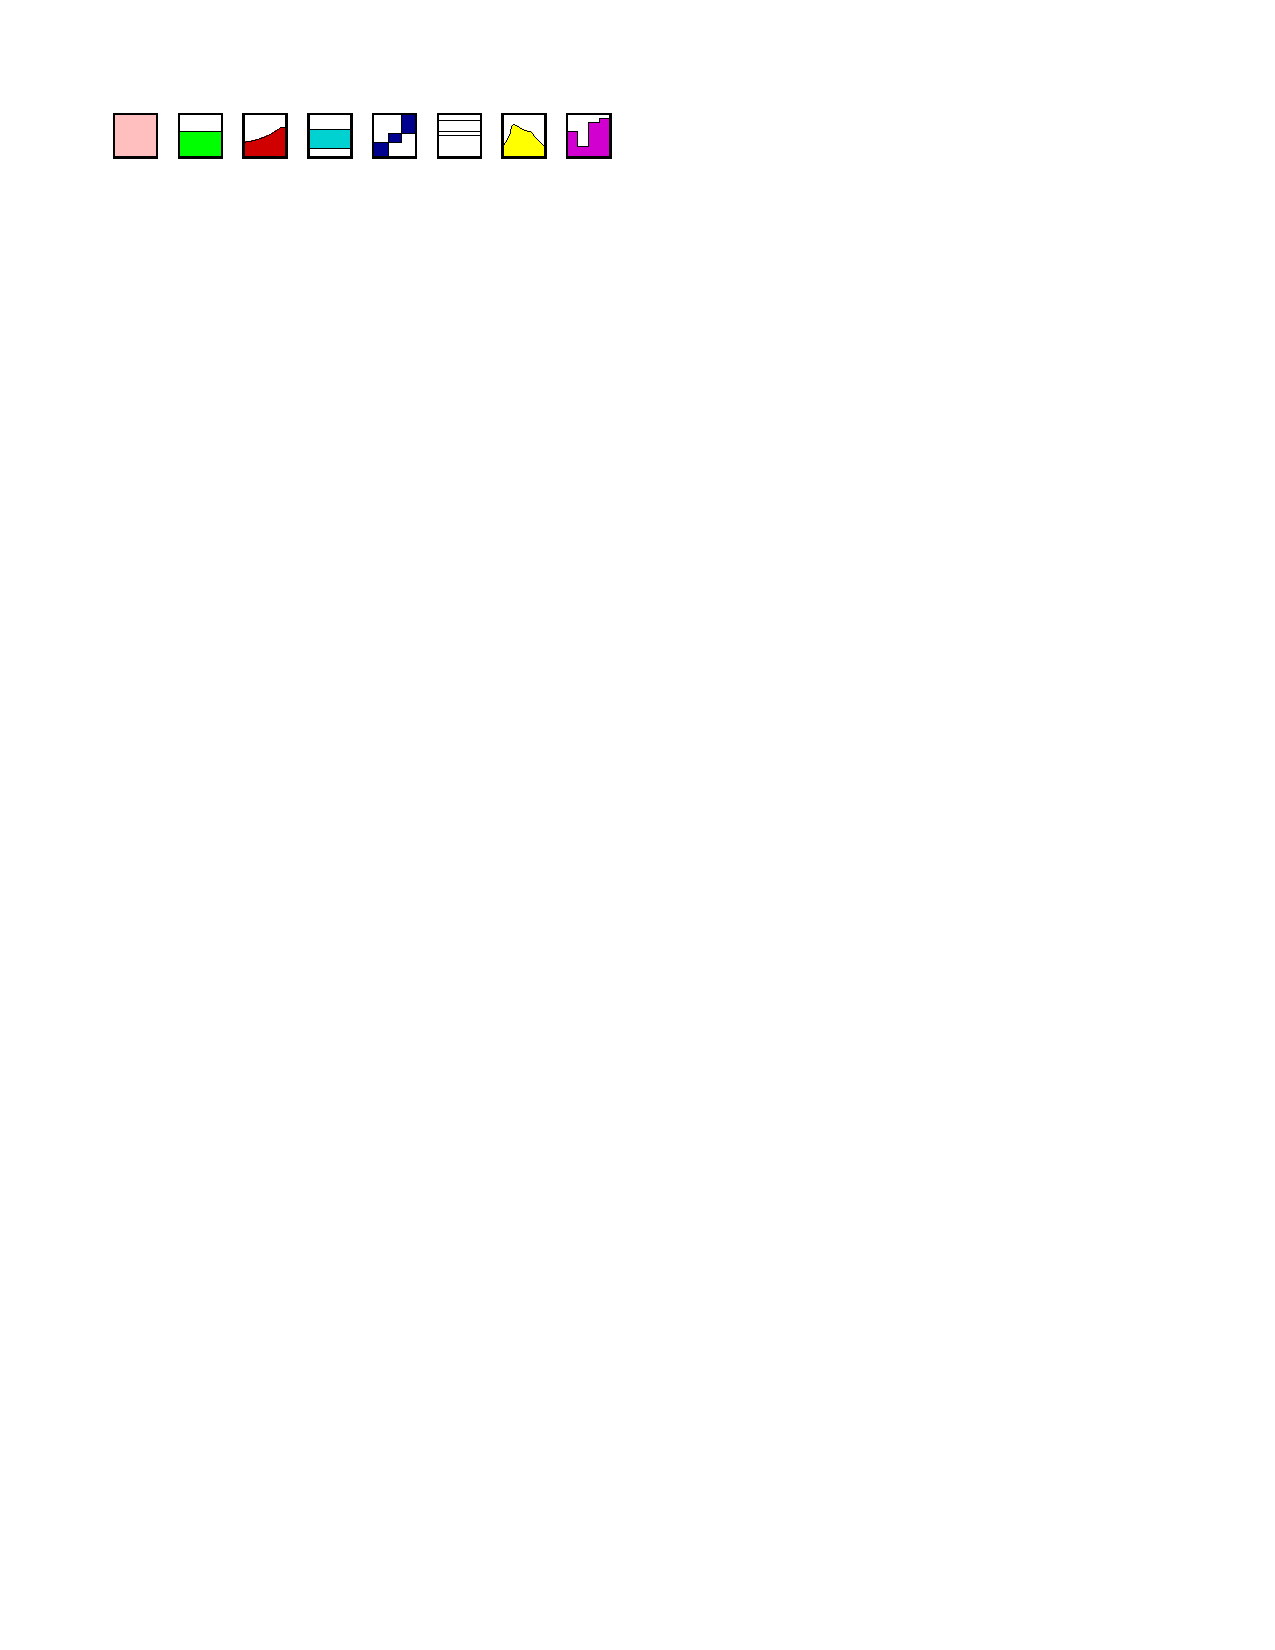
\includegraphics[width=0.65\textwidth]{figures/glyphs_zame.pdf}
    \caption{Eight different glyphs for aggregated edges (color shade,
average, min/max histogram, min/max range, min/max tribox, Tukey
box, smooth histogram, step histogram)~\cite{ElmqvistDGHF08}.}
    \label{fig:glyphs-zame}
  \end{center}
\end{figure}